\documentclass[12pt,titlepage]{article}
\usepackage[margin=1.0in]{geometry}
\usepackage{graphicx}
\usepackage[pdftex]{hyperref}
\usepackage[english]{babel}
\usepackage{csquotes}
\usepackage{titling}
\usepackage{titlesec}
\usepackage{xspace}
\usepackage{tabularx}
\usepackage{float}
\usepackage{parskip}

% Commands
% ========

% Names of things
% ---------------
\newcommand\protagonist{Vivian\xspace}
\newcommand\dad{Harrison\xspace}
\newcommand\mom{MOM\xspace}
\newcommand\hometown{TOWNSVILLE\xspace}
\newcommand\evilcorp{Iskandar\xspace}
\newcommand\world{KANTO\xspace}
\newcommand\cardgame{CARDGAME\xspace}

\newcommand\gametitle{\textit{\AE on Chronicles}\xspace}

% Useful things
% -------------

\newcommand\sep{\rule{2.5in}{0.1mm}}
\newcommand\tss{\textsuperscript}


\MakeOuterQuote{"}

\newcommand\tab[1][.5in]{\hspace*{#1}}

% http://tex.stackexchange.com/a/50186/100230
\newcommand{\subtitle}[1]{
    \posttitle{
    \par\end{center}
\begin{center}\large#1\end{center}
    \vskip0.5em
}
}

% http://tex.stackexchange.com/a/60212/100230
\titleclass{\subsubsubsection}{straight}[\subsection]

\newcounter{subsubsubsection}[subsubsection]
\renewcommand\thesubsubsubsection{\thesubsubsection.\arabic{subsubsubsection}}

\titleformat{\subsubsubsection}
{\normalfont\normalsize\bfseries}{\thesubsubsubsection}{1em}{}
\titlespacing*{\subsubsubsection}
{0pt}{3.25ex plus 1ex minus .2ex}{1.5ex plus .2ex}

\makeatletter
\renewcommand\paragraph{\@startsection{paragraph}{5}{\z@}%
    {3.25ex \@plus1ex \@minus.2ex}%
    {-1em}%
{\normalfont\normalsize\bfseries}}
\renewcommand\subparagraph{\@startsection{subparagraph}{6}{\parindent}%
    {3.25ex \@plus1ex \@minus .2ex}%
    {-1em}%
{\normalfont\normalsize\bfseries}}
\def\toclevel@subsubsubsection{4}
\def\toclevel@paragraph{5}
\def\toclevel@paragraph{6}
\def\l@subsubsubsection{\@dottedtocline{4}{7em}{4em}}
\def\l@paragraph{\@dottedtocline{5}{10em}{5em}}
\def\l@subparagraph{\@dottedtocline{6}{14em}{6em}}
\makeatother

\setcounter{secnumdepth}{4}
\setcounter{tocdepth}{4}

% http://tex.stackexchange.com/a/56558/100230
\AtBeginDocument{\renewcommand\contentsname{Table of Contents}}

\title{\gametitle}
\subtitle{SUBTITLE?}
\author{Team Epsilon}
\date{\today}

\begin{document}
\maketitle

\tableofcontents
\newpage
\listoffigures
\newpage
\listoftables

% NOTES:
% - There are some places where I have commented out a list of items that are suggested to be
%   included in the document. Make them subsections as necessary.
% - I basically copy pasta-d from Baldwin's template.

\newpage
\section{Design History}
% This is a change listing quickly describing each major version and changes.
\begin{table}[H]
    \caption{Version History}
    \label{tbl:version_history}
    \centering
    \begin{tabularx}{\linewidth}{| l | l || X |}
        \hline
        \textbf{Version Number} & \textbf{Date} & \textbf{Change Description} \\
        \hline\hline
        1.0 & 2017-02-03 & First Draft \\
        \hline
        2.0 & 2017-02-10 & Initial Design Completed \\
        \hline
    \end{tabularx}
\end{table}

\newpage
\section{Game Overview}
\gametitle is a story-based, adventure RPG inspired by [TODO: INSPIRATION AND
REFERENCE]. The game's theme is Aether punk. Blah blah blah.

\subsection{Game Concept}

\subsection{Feature Set}

\subsection{Genre}

\subsection{Target Audience}

\subsection{Game Flow Summary}
% How does the player move through the game. Both framing interface and the game
% itself.

During gameplay, the player will experience two primary views. The first is the
{\it overworld view}, where the player navigates the land of \world. In this
view, isometric projection of the game world centers on the playable character
as the player travels \world. The player can interact with the world's NPCs via
their sprites, enter buildings, and pick up items. Interactions with the NPCs
will often lead to \cardgame battles , which then switches the game interface to
the {\it combat view}.

The combat view is where \cardgame battles take place; the design is shown in
Figure \ref{fig:combat} of Section \ref{sec:concept_art}. This view consists of
a battle scene, which displays animations of the cards currently in play, with
the player's card animations on the left and enemy NPC's on the right.
Information about the game is communicated to the user through the surrounding
combat interface. This interface includes the HP of the player and opponent
(top-right), the player's card (bottom-center), stats for the currently selected
card (bottom-left), deck and remaining card count (bottom-right), and [TODO: NOT
SURE WHAT THAT IS ON THE TOP-LEFT] (top-left). Once the battle is over, the
player returns to the overworld view.

\subsection{Look and Feel}
% What is the basic look and feel of the game? What is the visual style?
IN PROGRESS: Aether Punk

\subsection{Project Scope}
% A summary of the scope of the game
%
% - Number of Locations
% - Number of Levels
% - Number of NPC's
% - Number of Weapons
% - etc.

There will be three cities outside of the main character's hometown, as well as
three themed non-city areas: a cave, a jungle, and a desolate wasteland. The
game will progress through the locations in the order:

\begin{enumerate}
    \item Hometown
    \item Cave
    \item City \#1
    \item Jungle
    \item City \#2
    \item Desolate Wasteland
    \item City \#3
\end{enumerate}

The final area is where the player confronts \evilcorp and faces their final
three opponents during the climax of the story. In each of the first two cities,
the player will have to defeat a single NPC to move on to the next section. In
each of the non-city areas, the player will have to complete three card battles
against NPCs, which will tend to be easier than the city battles. Further, each
city battle and one of each trio of non-city battles will reward the player with
one or more additional cards.

[TODO: NUMBER OF UNIQUE CARDS IN THE GAME]

\newpage
\section{Gameplay and Mechanics}

\subsection{Gameplay}

\subsubsection{Game Progression}

\subsubsection{Mission/Challenge Structure}

\subsubsection{Puzzle Structure}

\subsubsection{Objectives}
% What are the objectives of the game?

\subsubsection{Play Flow}
% How does the game flow for the game player?

\subsection{Mechanics}
% What are the rules to the game, both implicit and explicit.  This is the model
% of the universe that the game works under.  Think of it as a simulation of a
% world, how do all the pieces interact?  This actually can be a very large
% section.

\subsubsection{Physics}
% How does the physical universe work?

\subsubsection{Movement}
% - General Movement
% - Other movement

\subsubsection{Objects}
% - Picking up objects
% - Moving objects

\subsubsection{Actions}
% - Switches and Buttons
% - Picking up, Carrying and Dropping
% - Talking
% - Reading

\subsubsection{Combat}
% If there is a combat or even conflict, how is this specifically modeled?

\subsubsection{Economy}
% What is the economy of the game? How does it work?

\subsection{Screen Flow}

\subsubsection{Screen Flow Chart}
% A graphical description of how each screen is related to every other

\subsubsection{Screen Descriptions}
% What is the purpose of each screen?
%
% - Main menu screen
% - Options screen
% - etc.

\subsection{Game Options}
% What are the options and how do they affect gameplay and mechanics?

\subsection{Replaying and Saving}

\subsection{Cheats and Easter Eggs}

\newpage
\section{Story, Setting, and Character}

The story is centered around a single character, \protagonist, who embarks on an
adventure to save her parents, \dad and \mom, from the evil clutches of
\evilcorp. Join \protagonist as she makes her way across the land of \world to
face \evilcorp head-on and save her parents!

\subsection{Story and Narrative}

The narrative is communicated as dialogue between characters, though
supplemental non-dialogue narrative will be provided when necessary (primarily
during the introduction and final exposition). The perspective will never leave
that of \protagonist so that the player only knows what \protagonist discovers
throughout the quest.

\subsubsection{Back Story}

A young girl lives in a modest but loving household with her two parents. Her
parents think of her as their world, and she loves both of her parents very
much.

Her parents are inventors, a skill which the girl always felt had not been
passed down the genetic line. Their inventing skills were used to supply the
town with creative solutions to minor problems. They had not been particularly
successful in breaking into a larger industry; their ideals against intellectual
property kept them out of the larger corporations. Besides, they were perfectly
content in their small town with their friends and a seemingly interminable
stream of minor problems for them to solve.

They do, however, have one major project that they collaborate with
inventors-of-similar-ideals on: the very first free and open-source brain
augmentation platform.

\sep

Brain augmentation was not a new technology. The first feasible attempts at its
implementation had begun 150 years prior to the present day, with success
initially achieved by NeuroTransmission Labs. Unfortunately, due to the
proprietary nature of its design and specialized hardware, it was only
accessible to the richest of the world's citizens; not even the average employee
at NeuroTransmission Labs was granted use of the technology.

As with any consumer good in history, it was expected that competition combined
with advances in hardware production would steadily lower the price until even
the lower-middle class would have access to older, yet still revolutionary,
versions of the brain augmentation platform. This claim turned out to be
incorrect. Those fortunate enough to have access to brain augmentation began to
form their own branch of social mentality: rather than allow the platform to
trickle down to the masses, they thought it better to restrict its use as much
as possible. Vast improvements continued to be made to the technology initiated
by NeuroTransmission Labs, while out-of-date models were either destroyed or
saved for future research.

50 years after the inception of brain augmentation technology, a test was
conducted by its proprietors: a controlled release of a restricted model,
specifically geared toward qualified infants whose parents were able to pass an
'ingenuity test'. 50,000 lucky participants were selected out of the nearly 1
million infants initially considered. The acceleration of this subset of the
general population had an astounding effect: the already-unprecedented
socioeconomic gap shot open, a wound that left the already poor and starving
citizens with even less hope than they thought possible. This experiment is 
known as the Aeon Project.

\subsubsection{Plot Elements}


\subsubsection{Game Progression}

One day, the girl's house is set on fire. She rushes to find her parents, who
are nowhere to be found. The final place she looks is her parents' workshop, but
still no sign. As she leaves the workshop, she makes the quick decision to grab
one of her parents' inventions before the fire destroys them all and her old
life.

A bit of thought and investigation leads the girl to believe that her parents
were taken by the corporation who were bent on stopping the development of
open-source brain augmentation technology for the masses. The girl then goes on
a quest to rescue her parents, traveling through the land and engaging in card
battles to survive and become strong enough to fight whatever lies ahead.

Finally, she reaches the corporations' HQ and fights the final battle...

\subsubsection{License Considerations}

\subsubsection{Cut Scenes}

\subsubsubsection{Cut Scene \#1}
% - Actors
% - Description
% - Storyboard
% - Script

\subsubsubsection{Cut Scene \#2}

% more cut scenes as necessary

\subsection{Game World}

\subsubsection{General Look and Feel}

\subsubsection{Area \#1}
% - General description
% - Physical Characteristics
% - Levels that use area
% - Connections to other areas

% more areas as necessary

\subsection{Characters}

\subsubsection{Vivian}
% - Back story
% - Personality
% - Look
%       - Physical Characteristics
%       - Animation
% - Special Abilities
% - Relevance to game story
% - Relationship to other characters
% - Statistics

% more characters as necessary

\subsubsection{Rosalind}
\tab Rosalind was born into a wealthy family. She is about the same age as Vivian, 
but because they grew up in such different environments, they see the world from 
opposite ends of the spectrum. Her parents are quite strict and often away, which 
has made Rosalind into a very independent and slightly socially isolated person. 
Her disconnect with her family has led her to crave something more, so she 
decides to experiment with brain augmentation technology. The technology 
improves upon some of her already developed personal strengths. She is very 
good at problem-solving, and the brain augmentation heightens her senses, most 
noticeably her hearing. Her personality is reserved. She manages herself well and 
knows how to get her way, but what she really craves is someone who she can 
talk to and spend time with. She doesn't pity the poor, but she feels some guilt 
about having access to the brain augmentation technology while others do not. 
Rosalind is blonde with long, wavy hair and steely grey eyes. Due to the 
augmentation, Rosalind has become more attuned with the Aether in the world, 
allowing her to use psionic like abilities. Etc..... more to come

As one of the 50,000 infants to have been chosen during the Aeon Project, 
Rosalind has become attuned to the Aether in the world. She developed enhanced 
strength and intelligence at a young age. As she grew older, she discovered that 
she could hear things exceptionally well, so well in fact that she could hear others 
thoughts

\subsubsection{Character \#3}

\newpage
\section{Levels}

\subsection{Level \#1}

\subsubsection{Synopsis}

\subsubsection{Introductory Material}
% Cut scene?  Mission briefing?

\subsubsection{Objectives}

\subsubsection{Physical Description}

\subsubsection{Map}

\subsubsection{Critical Path}

\subsubsection{Encounters}

\subsubsection{Level Walkthrough}

\subsubsection{Closing Material}

% more levels as necessary

\newpage
\section{Interface}

\subsection{Visual System}

\subsubsection{HUD}
% What controls?

\subsubsection{Menus}

\subsubsection{Rendering System}

\subsubsection{Camera}

\subsubsection{Lighting Models}

\subsection{Control System}
% How does the game player control the game? What are the specific commands?

\subsection{Audio}

\subsection{Music}

\subsection{Sound Effects}

\subsection{Help System}

\newpage
\section{Artificial Intelligence}

\subsection{Opponent AI}
% The active opponent that plays against the game player and therefore requires
% strategic decision making (example, Civilization or Chess, how is it to be
% designed?)

\subsection{Enemy AI}
% Villains and Monsters

\subsection{Non-combat Characters}


\subsection{Friendly Characters}

\subsection{Support AI}

\subsubsection{Player and Collision Detection}

\subsubsection{Pathfinding}

\newpage
\section{Technical}
% This may be an abbreviated of most of the Technical Bible
%
% - Target Hardware
% - Development hardware and software
% - Development procedures and standards
% - Game Engine
% - Network
% - Scripting Language
% - etc.

Team Epsilon will develop \gametitle on Windows using the following tools:

\begin{itemize}
    \item GameMaker game engine
    \item Photoshop for creating electronic artwork
    \item Visual Studio for implementing game physics and other complex logic
    \item FL Studio 12 for creating sounds and music
\end{itemize}

The team will use Game Maker Language and C++ for the game logic.

\sep

Players of \gametitle will need computers with the following minimum
specifications:

\begin{itemize}
    \item Windows (XP or later)
    \item 1 GB RAM
    \item 1 GB Free Space on Hard Disk
    \item 128 MB Graphics
    \item $1024 \times 600$ resolution
\end{itemize}

\newpage
\section{Game Art}
% This may be abbreviated with most of the content in an Art Bible
%
% - Concept Art
% - Style Guides
% - Characters
% - Environments
% - Equipment
% - Cut scenes
% - Miscellaneous

\subsection{Concept Artwork}\label{sec:concept_art}

\begin{figure}[H]
    \caption{Overworld View}
    \label{fig:overview}
    \centering
    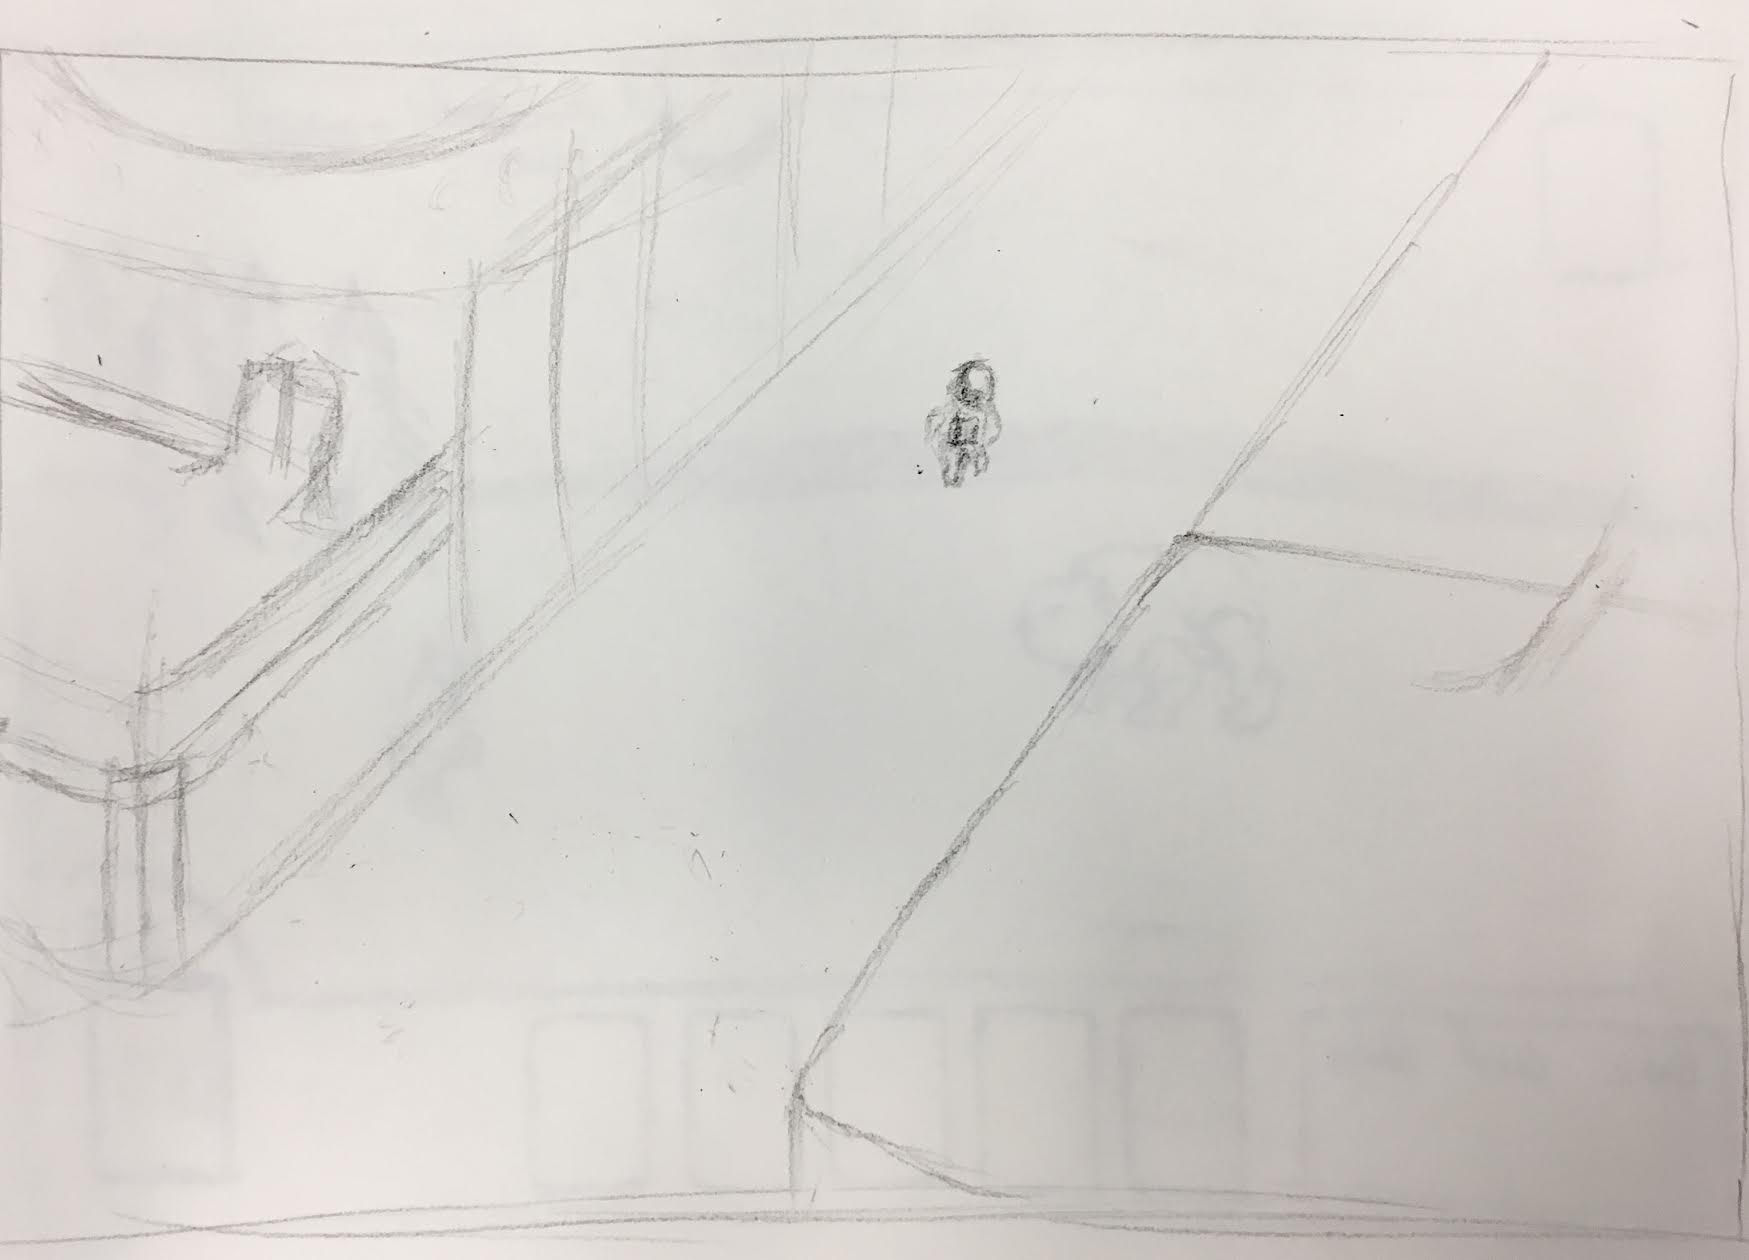
\includegraphics[width=0.7\textwidth]{../../graphics/overview}
\end{figure}

\begin{figure}[H]
    \caption{Combat View}
    \label{fig:combat}
    \centering
    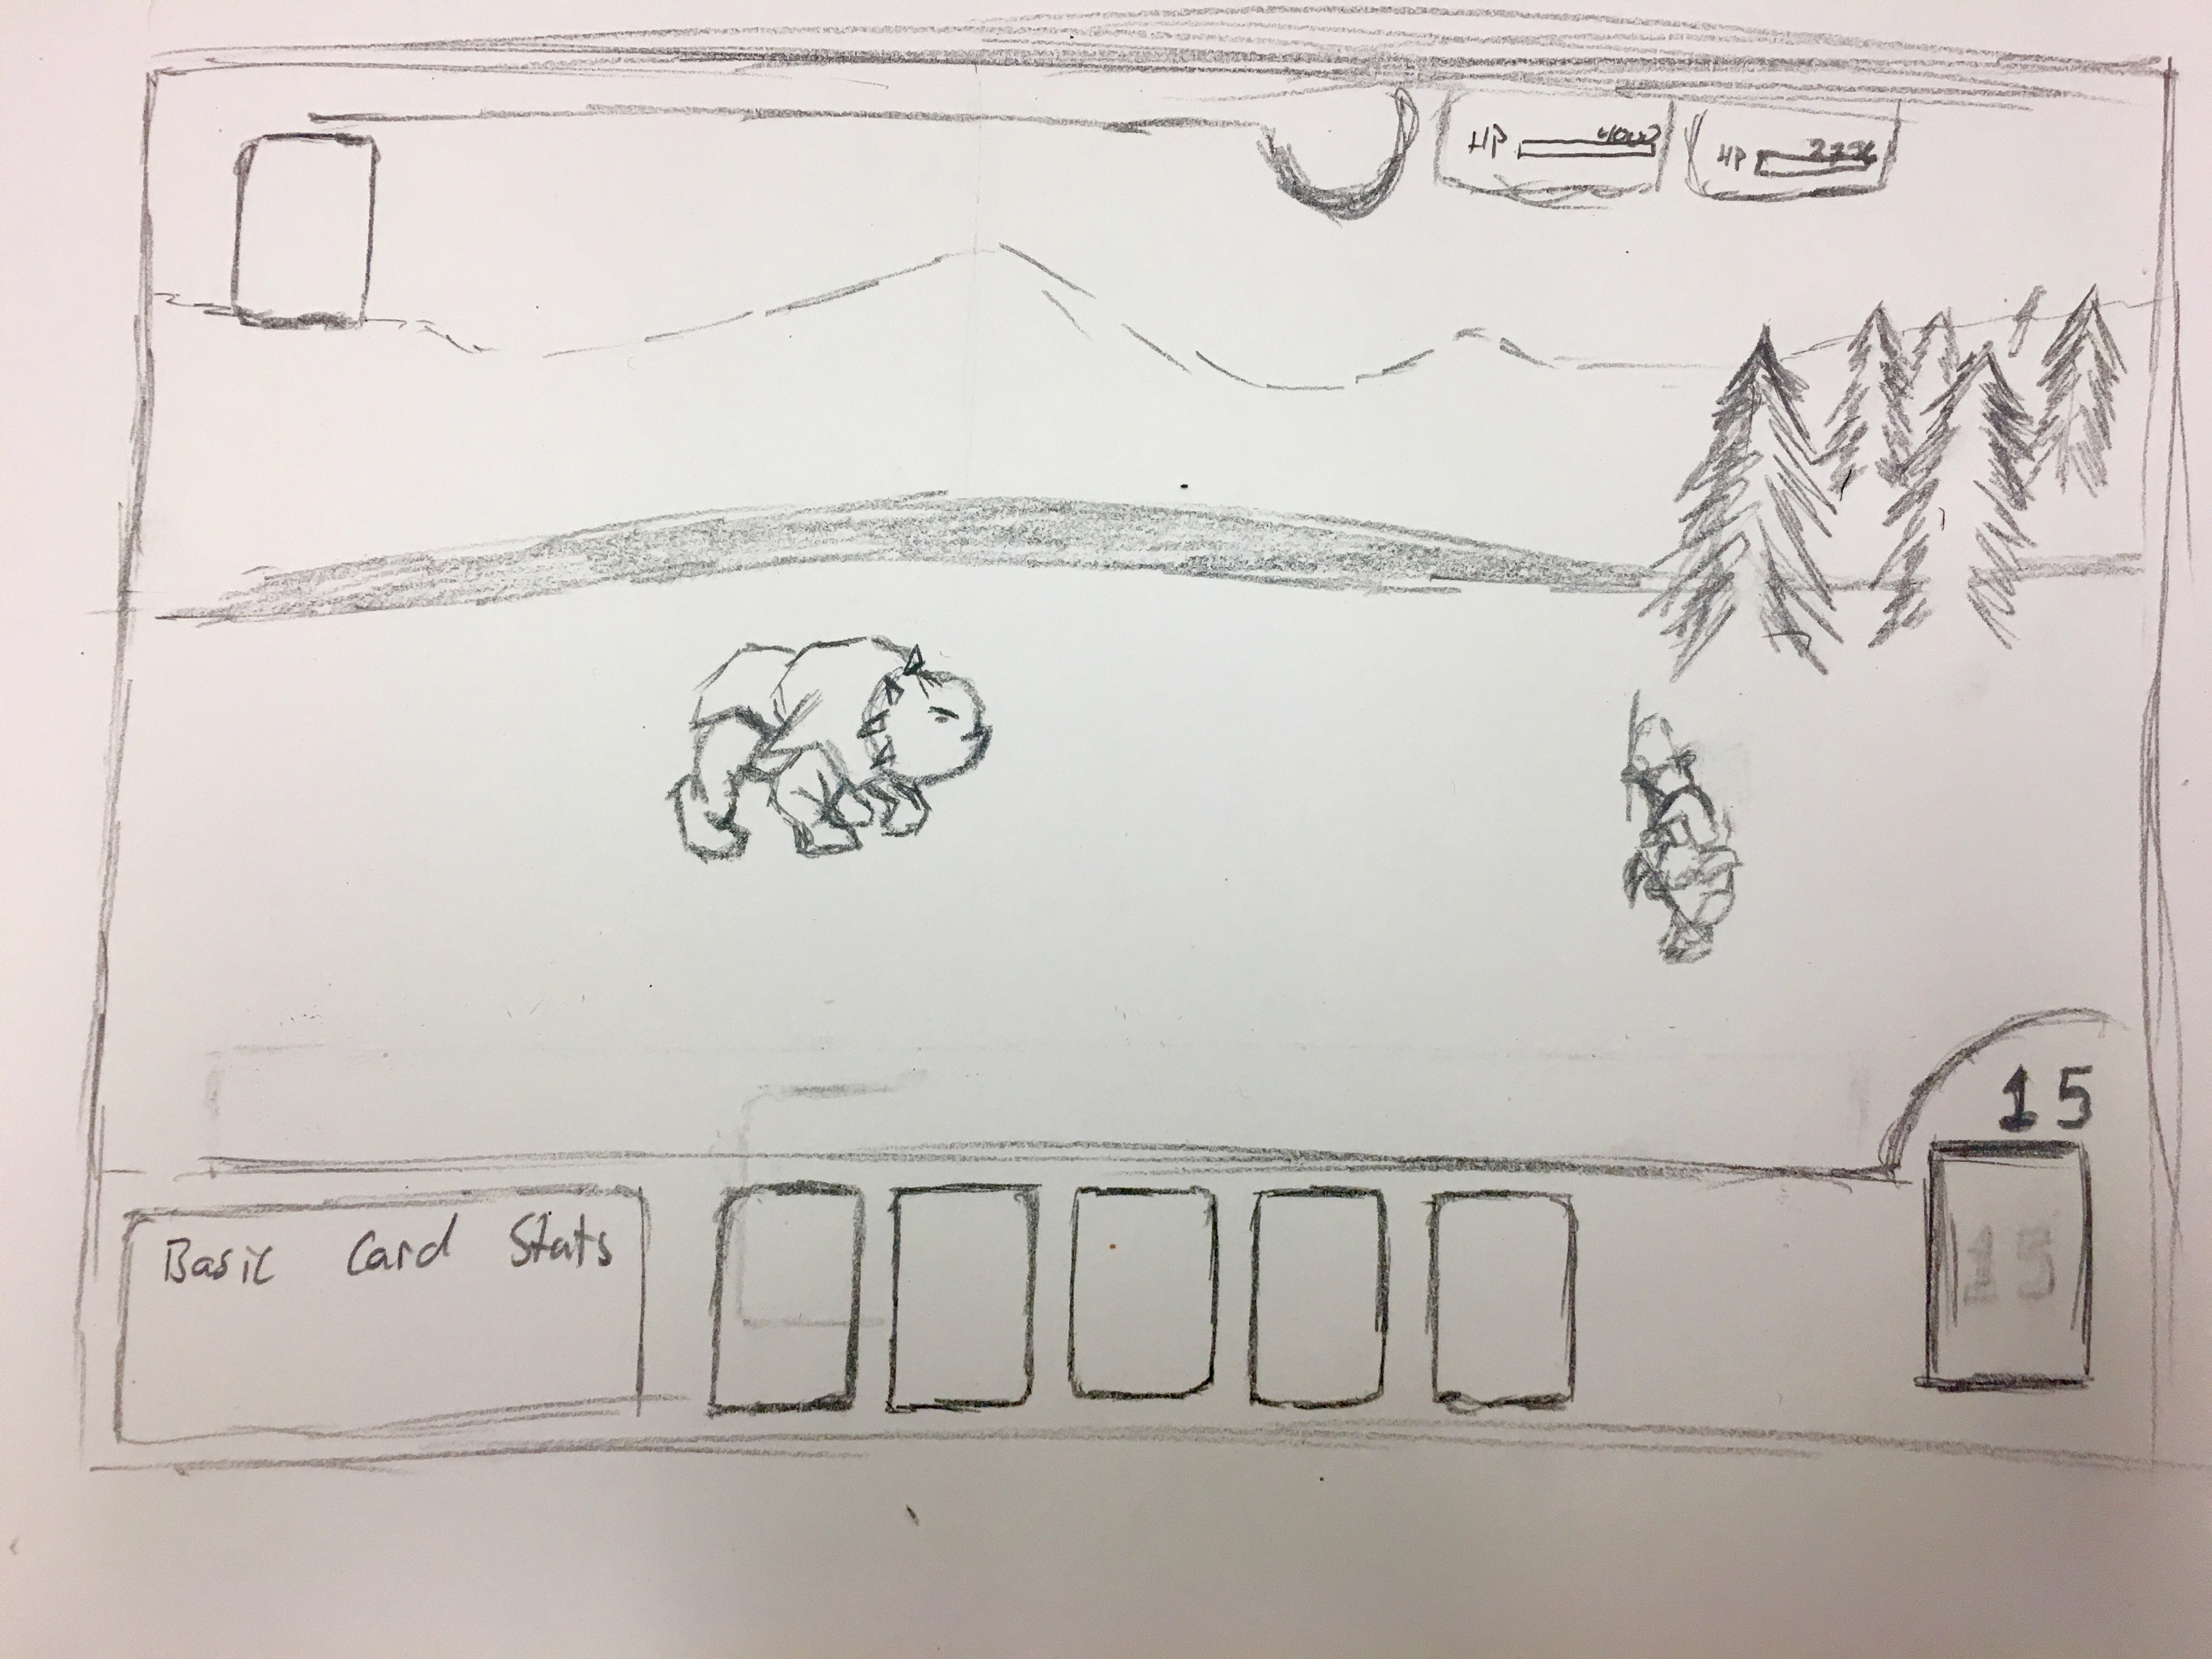
\includegraphics[width=0.7\textwidth]{../../graphics/combat}
\end{figure}

\begin{figure}[H]
    \caption{Weapon Concept}
    \label{fig:weapon_concept}
    \centering
    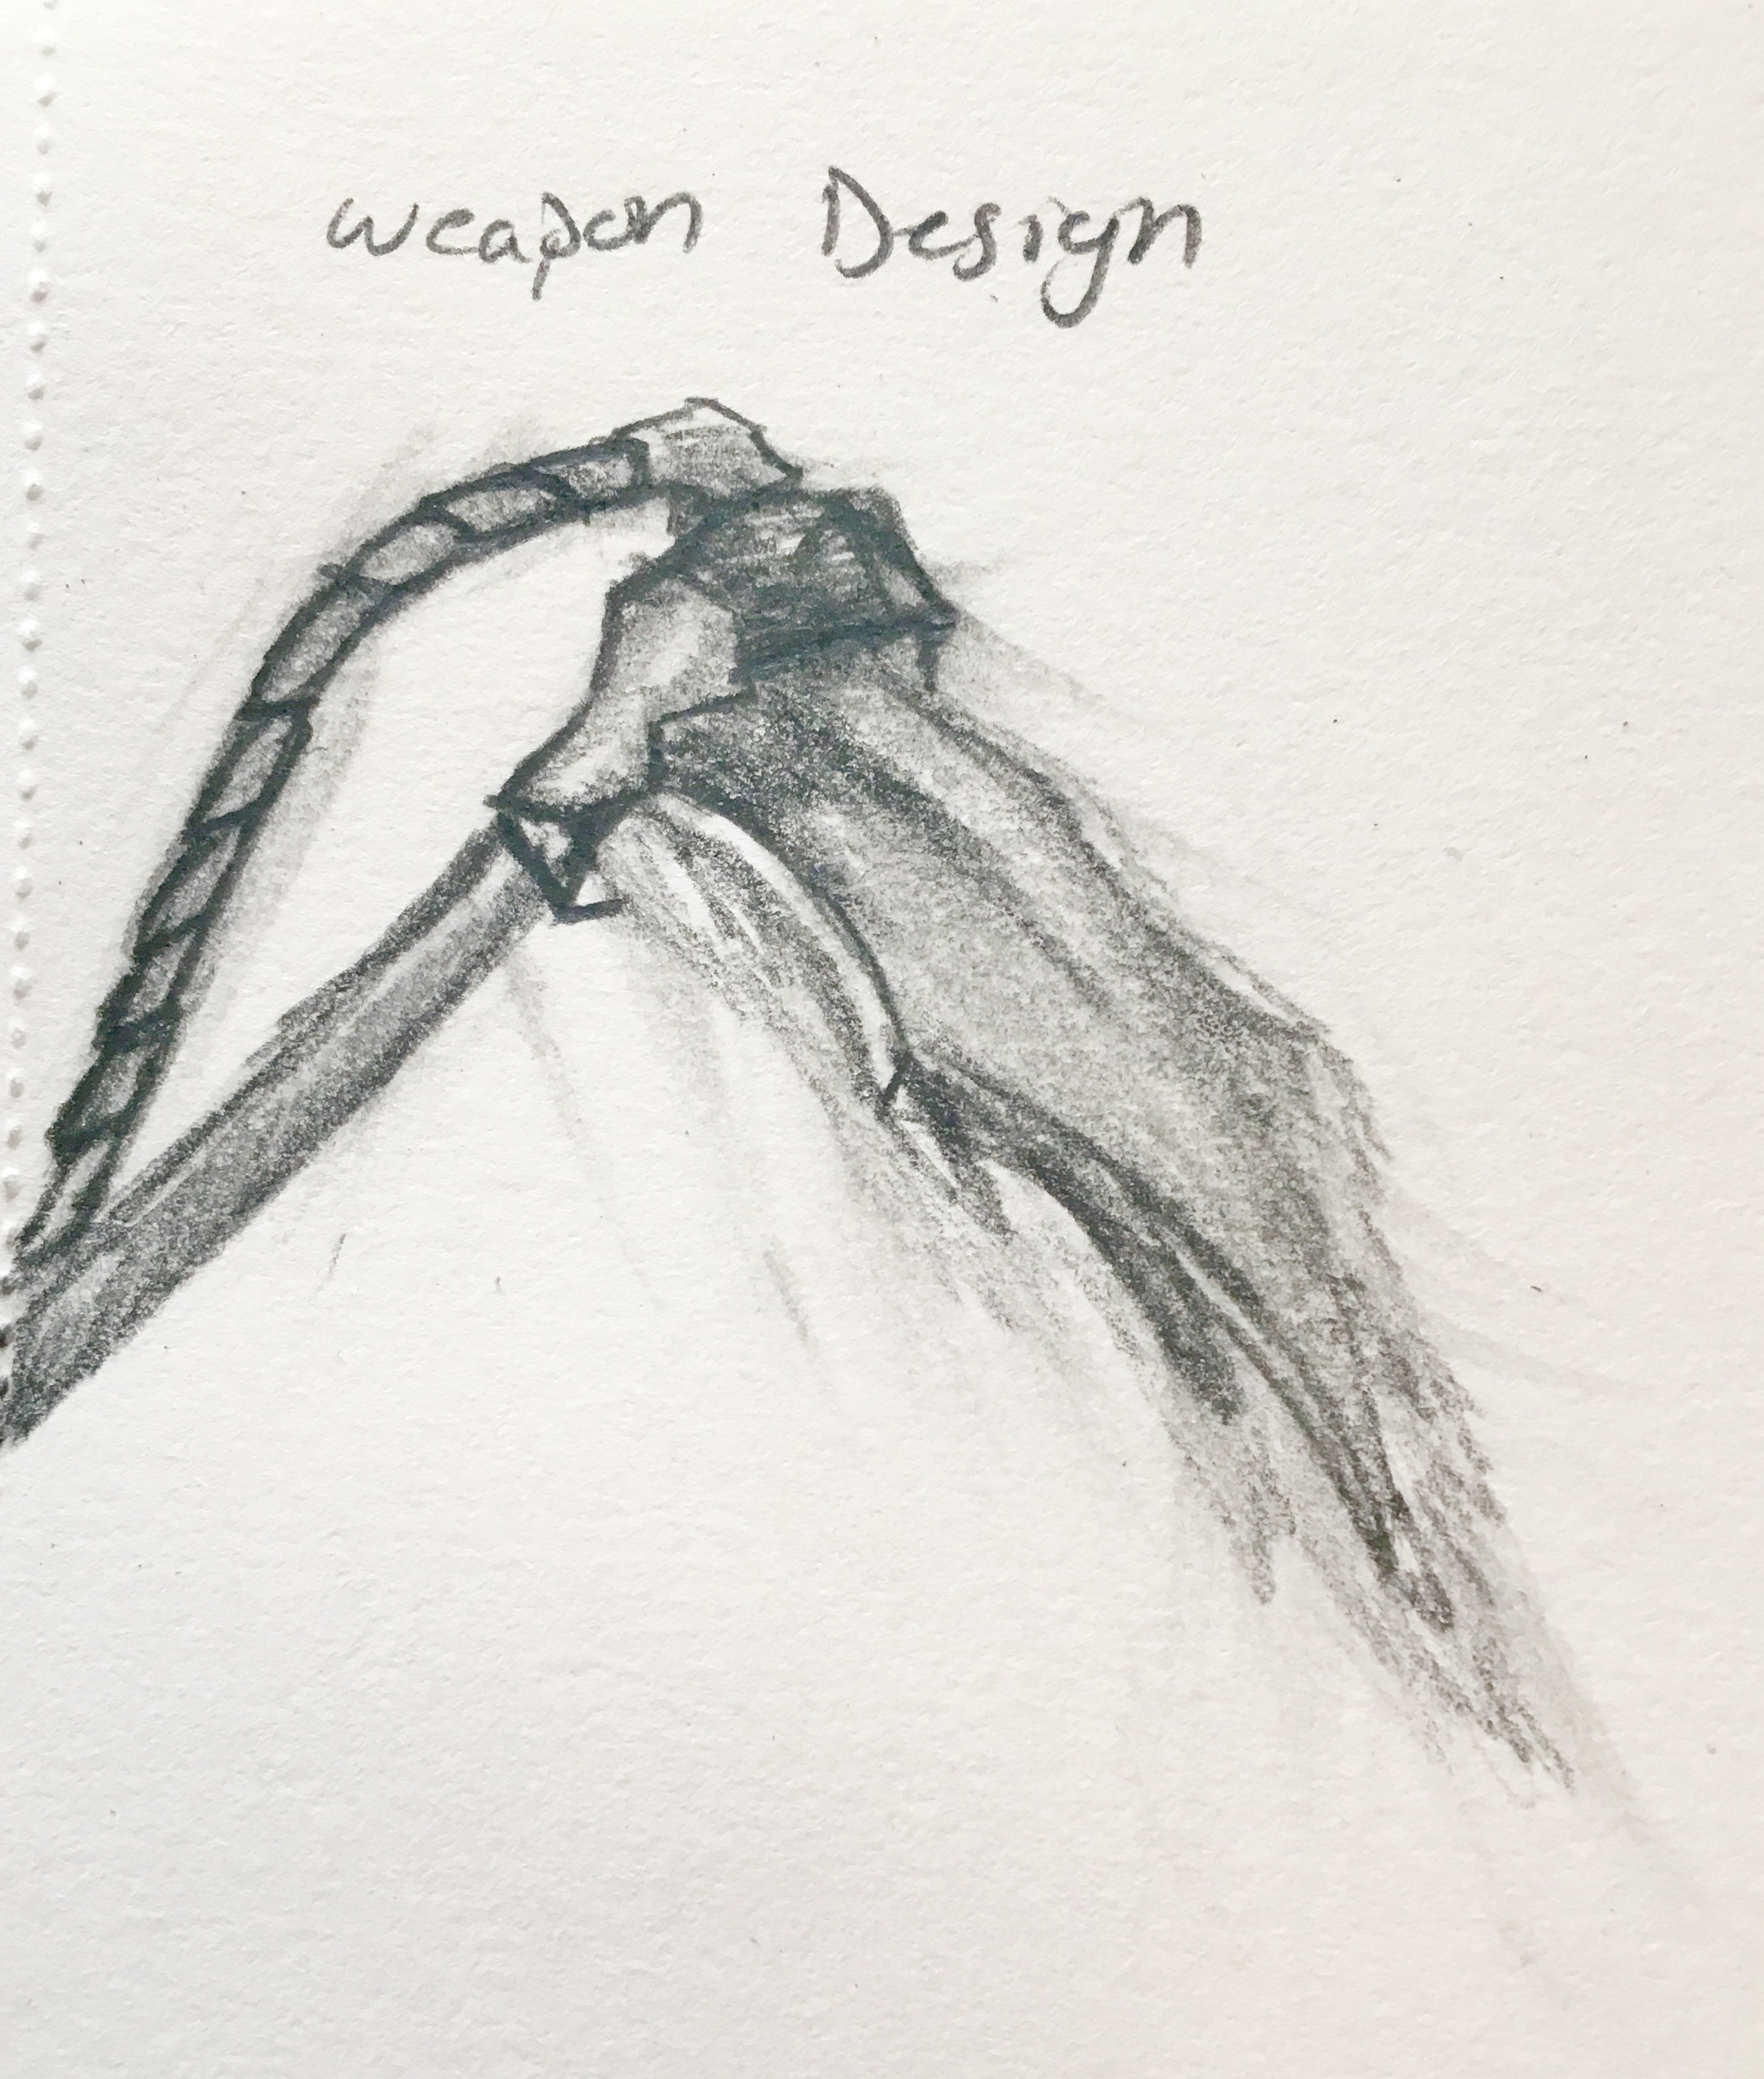
\includegraphics[width=0.35\textheight]{../../graphics/scythe}
\end{figure}

\begin{figure}[H]
    \caption{Enemy Concept}
    \label{fig:enemy_concept}
    \centering
    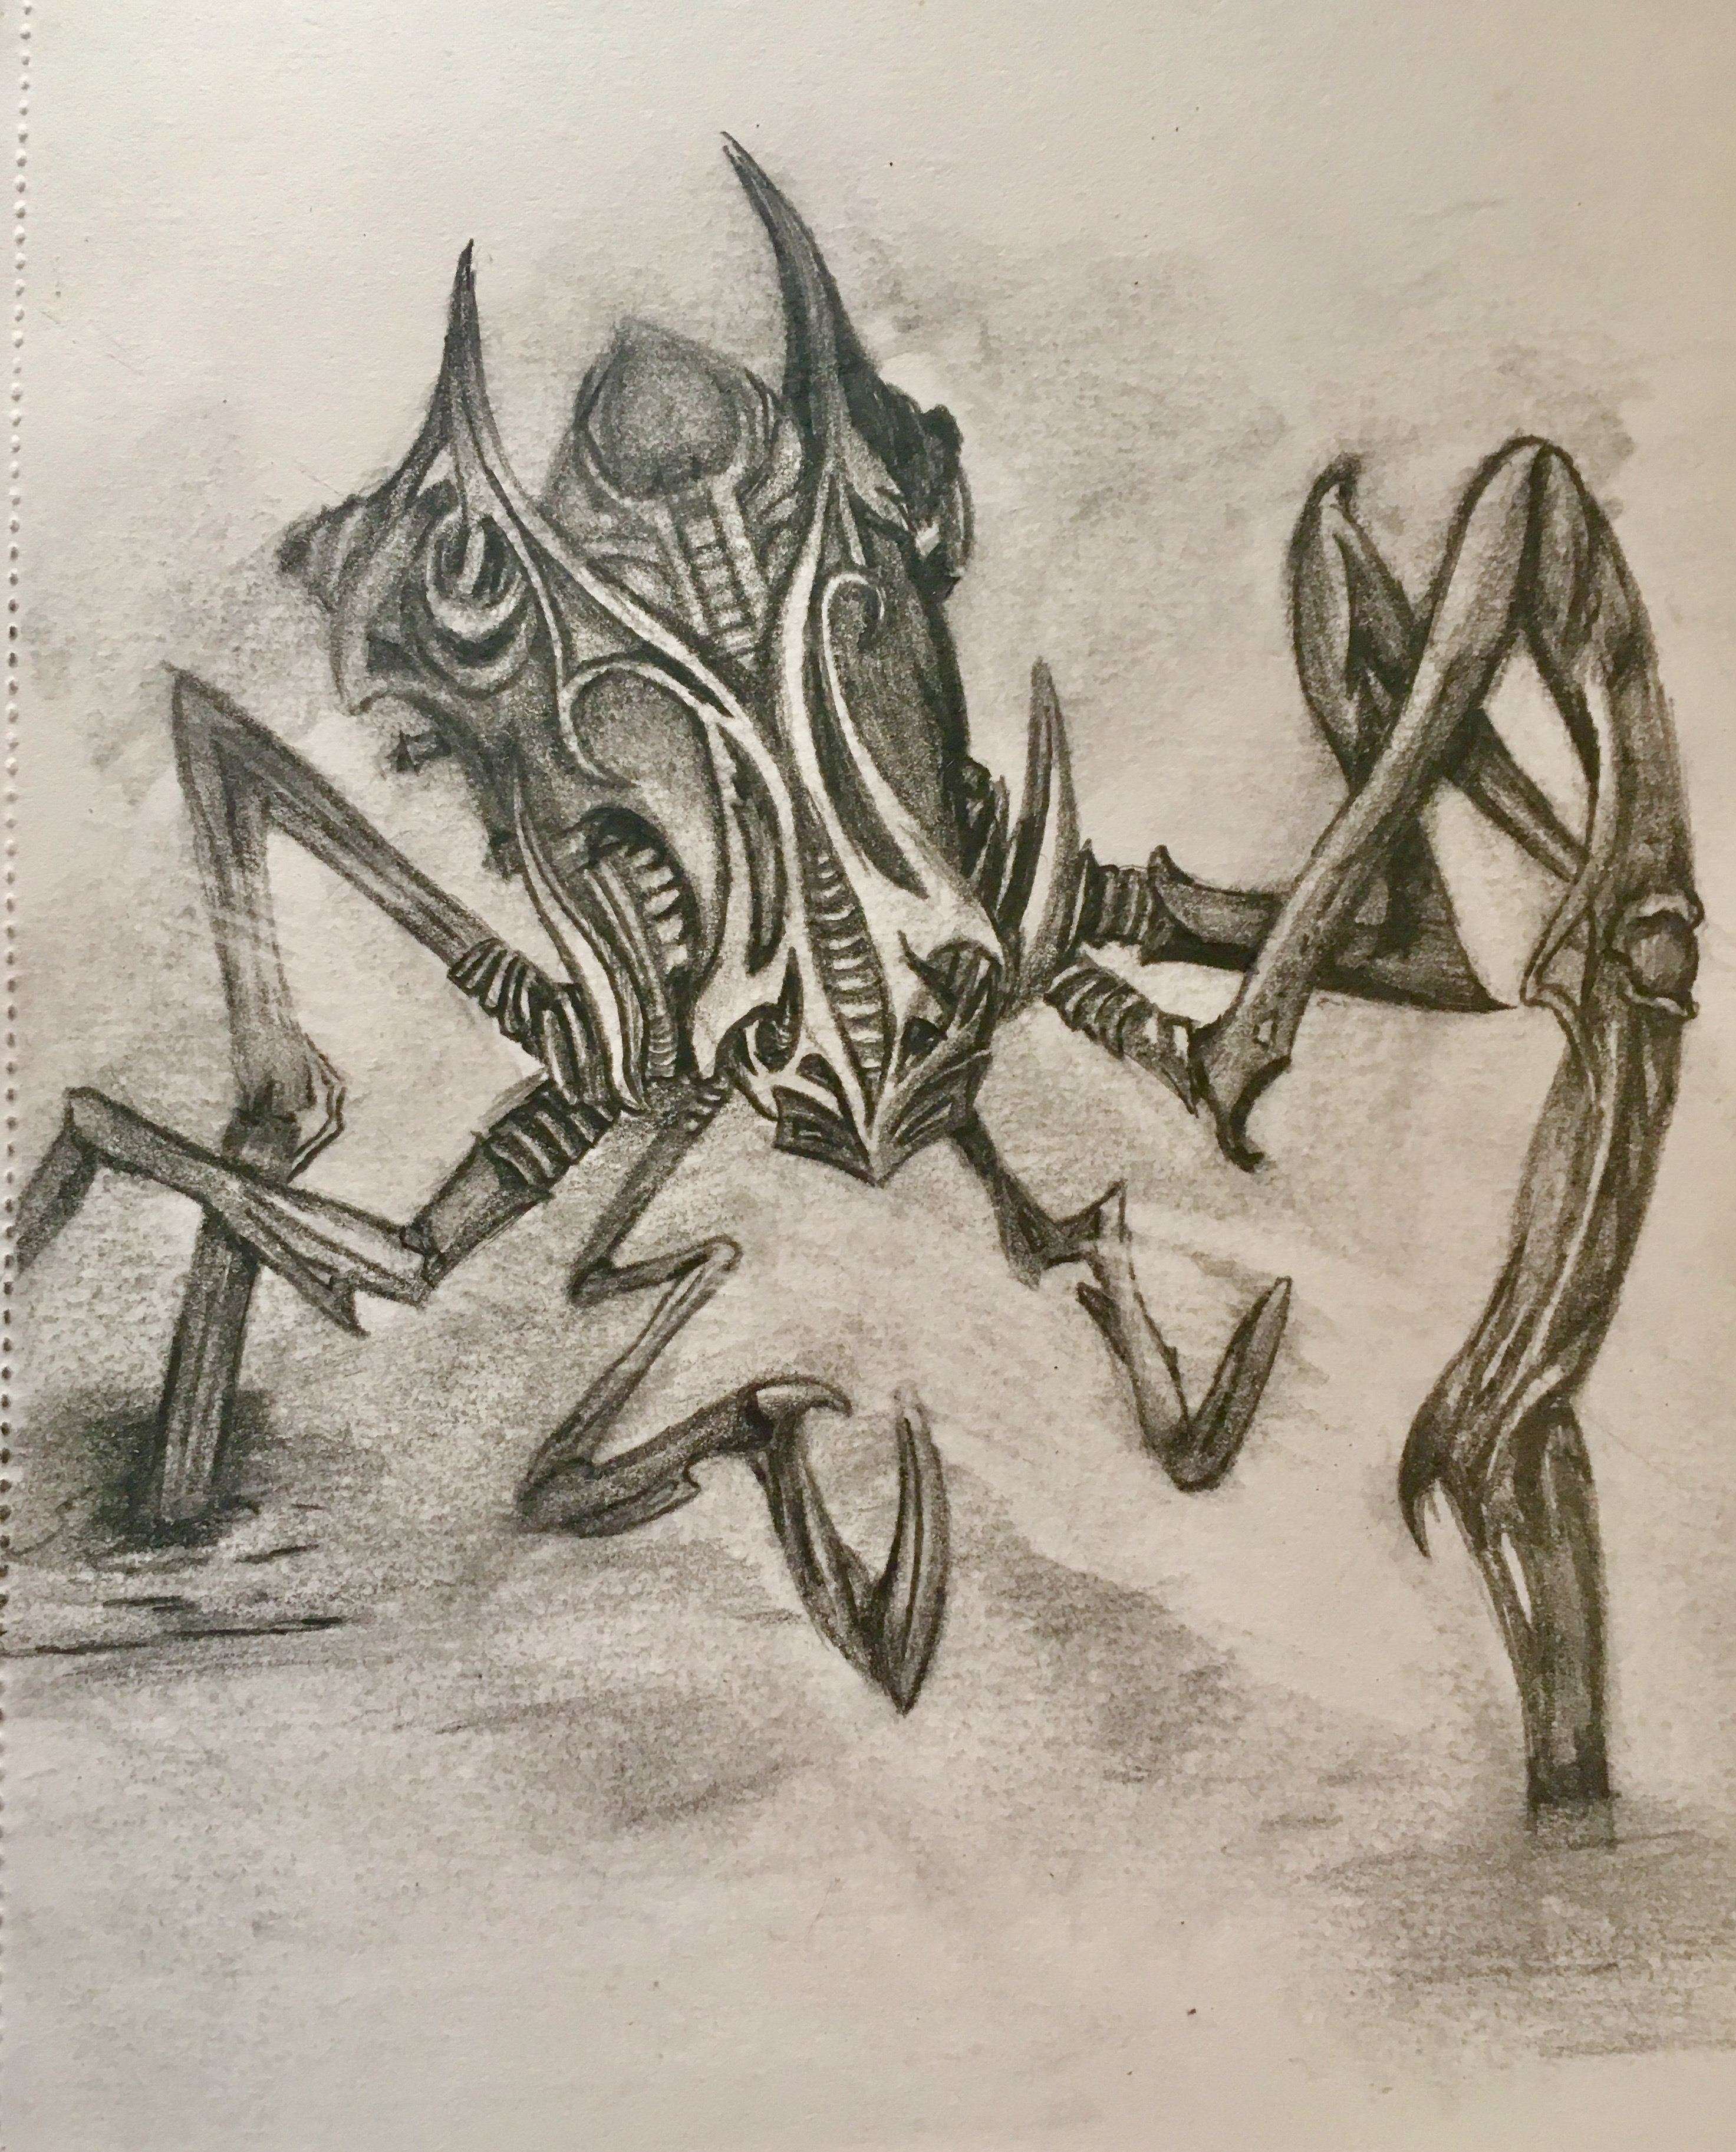
\includegraphics[width=0.35\textheight]{../../graphics/spider}
\end{figure}

\newpage
\section{Secondary Software}
% Editor, Installer, Update Software

\newpage
\section{Management}

\subsection{Detailed Schedule}
Table~\ref{tab:milestones} shows the five major milestones and their due dates.
\begin{table}[H]
    \caption{Milestone Delivery Schedule}
    \label{tab:milestones}
    \centering
    \begin{tabular}{|l|l|}
        \hline
        \textbf{Milestone} & \textbf{Date} \\
        \hline\hline
        Milestone I: Overworld & 2017/02/27 \\
        \hline
        Milestone II: Combat & 2017/03/13 \\
        \hline
        Milestone III: Alpha & 2017/03/24 \\
        \hline
        Milestone IV: Beta & 2017/04/14 \\
        \hline
        Milestone V: Final & 2017/04/26 \\
        \hline
    \end{tabular}
\end{table}

% TODO: More details

\subsection{Budget}
Given the expenses from Table~\ref{tab:expenses} and including a small buffer
for unforeseen expenses, production and marketing of \gametitle will cost \$6
million.

\begin{table}[H]
    \caption{Expenses}
    \label{tab:expenses}
    \centering
    \begin{tabular}{|l|r|}
        \hline
        \textbf{Item} & Amount \\
        \hline\hline
        \textbf{Labour} & \textbf{\$500,000} \\
        \tab Caleb & \$100,000 \\
        \tab David & \$100,000 \\
        \tab Jacob & \$100,000 \\
        \tab Robbie & \$100,000 \\
        \tab Sumner & \$100,000 \\
                    &\\
        \textbf{Equipment} & \textbf{\$6,193} \\
        \tab FL Studio 12 & \$99 \\
        \tab MSDN Standard Subscriptions (5) & \$5,995 \\
        \tab Adobe Creative Cloud & \$99 \\
                                  & \\
        \textbf{Travel} & \textbf{\$9,245} \\
        \tab San Francisco Game Developers Conference Tickets (5) & \$8,495 \\
        \tab Denver $\leftrightarrow$ San Francisco Plane Fare (5) & \$750 \\
                                                                   & \\
        \textbf{Marketing} & \textbf{\$5,212,000} \\
        \tab Ad Production & \$200,000 \\
        \tab Super Bowl Ad & \$5,000,000 \\
        \tab YouTube Ads & \$2,000 \\
        \tab Promotional Website & \$10,000 \\
        \hline\hline
        \textbf{TOTAL} & \textbf{\$5,727,438} \\
        \hline
    \end{tabular}
\end{table}

\subsection{Risk Analysis}

Table~\ref{tab:risks} lists all possible major risks of the project and
our contingency plans to avoid each issue and what we will do in the case that
it occurs.

\begin{table}[H]
    \caption{Risk Analysis}
    \label{tab:risks}
    \centering
    \begin{tabularx}{\linewidth}{|l|X|}
        \hline
        \textbf{Possible Risk} & \textbf{Contingency Plan} \\
        \hline
        Non-competitive enemy AI & If it proves too difficult to create
        different AIs for various enemies and bosses, we can opt to create
        only one enemy AI to use with every combat encounter. We can also
        make this more simple than we'd like to save time. \\
        \hline
        Overambitious project scope & We believe that we have allocated our
        milestone goals in a way that we will be able to implement the core
        gameplay and assets that are necessary for the game to function;
        however, it is possible that we have been overambitious in our
        allocations. If that is the case we will have to cut back on
        functionalities and assets starting with in depth art and music assets
        followed by unique cards and encounters in tandem with overworld
        locations and interactions. This could also limit story development.  \\
        \hline
        Meeting deadlines & This risk has many similarities to the risk of an
        overambitious project scope. If we are unable to integrate a desired
        functionality before a milestone delivery, we will table the
        functionality until we have extra time to complete it in addition to
        all other parts of the next delivery. This could result in it being
        tabled indefinitely in which case we will refer to the order of
        functionalities to drop described above. \\
        \hline
        Large number of dependencies between tasks & We believe we have
        allocated our milestone goals in a way that we will be able to
        implement the necessary functionalities prior to when we plan to
        implement the functionalities that depend on them. If that is not the
        case, similarly to the case of not meeting deadlines, we will drop
        functionalities in the order described above. \\
        \hline
    \end{tabularx}
\end{table}

\subsection{Test Plan}

In general, periodic plays and replays of sections of the game should be done to
provide a loose redundant check on the game's stability. A more formal testing
structure is defined next.

Testing of the game will take place in incremental steps throughout development
of the game. While automated testing would present a robust and consistent
testing method, the time constraints of the project and its nature as a video
game make this an infeasible testing strategy. Therefore, the team will rely on
a system of collaborative manual testing that works as follows:

\begin{enumerate}
    \item When adding a new feature to the game, the developer(s) adding the feature
        will test it and ensure that all directly affected aspects of the game
        perform in the expected manner. The feature will then be documented in the
        {\it Bugs \& Features} document. Any remaining bugs that the developer is
        unable to resolve should also be documented in the {\it Bugs \& Features}
        document.
    \item It is then up to the Test Lead to monitor the {\it Bugs \& Features}
        document for new features that they should test for completeness and bugs.
        If the Test Lead is unable to resolve all bugs for any reason, they may
        delegate specific bug resolutions to other members of the team.

        {\it Caveat}: In the case that the Test Lead has added a particular
        feature themselves, they must act in accordance with step 1. The task of
        further testing (step 2) then falls on the Team Leader by default, though
        the Test Lead may assign this to another team member at their own
        discretion on a case-by-case basis.
\end{enumerate}

\newpage
\section{Appendices}

\subsection{Asset list}

\subsubsection{Art}

\subsubsubsection{Model and Texture List}

\subsubsubsection{Animation List}

\subsubsubsection{Effects List}

\subsubsubsection{Interface Art List}

\subsubsubsection{Cut scene List}

\subsubsection{Sound}

\subsubsubsection{Environmental Sounds}

\subsubsubsection{Weapon Sounds}

\subsubsubsection{Interface Sounds}

\subsubsection{Music}

\subsubsubsection{Ambient}

\subsubsubsection{"Action"}

\subsubsubsection{Victory}

\subsubsubsection{Defeat}
% Etc.

\end{document}
